%package list
\documentclass{article}
\usepackage[top=3cm, bottom=3cm, outer=3cm, inner=3cm]{geometry}
\usepackage{graphicx}
\usepackage{url}
%\usepackage{cite}
\usepackage{hyperref}
\usepackage{array}
%\usepackage{multicol}
\newcolumntype{x}[1]{>{\centering\arraybackslash\hspace{0pt}}p{#1}}
\usepackage{natbib}
\usepackage{pdfpages}
\usepackage{multirow}
\usepackage{multirow}
\usepackage[normalem]{ulem}
\useunder{\uline}{\ul}{}


%%%%%%%%%%%%%%%%%%%%%%%%%%%%%%%%%%%%%%%%%%%%%%%%%%%%%%%%%%%%%%%%%%%%%%%%%%%%
%%%%%%%%%%%%%%%%%%%%%%%%%%%%%%%%%%%%%%%%%%%%%%%%%%%%%%%%%%%%%%%%%%%%%%%%%%%%
\newcommand{\csemail}{vmachacaa@ulasalle.edu.pe}
\newcommand{\csdocente}{MSc. Vicente Enrique Machaca Arceda}
\newcommand{\cscurso}{Compiladores}
\newcommand{\csuniversidad}{Universidad La Salle}
\newcommand{\csescuela}{Escuela Profesional de Ingeniería de Software}
\newcommand{\cspracnr}{02}
\newcommand{\cstema}{Introducción}
%%%%%%%%%%%%%%%%%%%%%%%%%%%%%%%%%%%%%%%%%%%%%%%%%%%%%%%%%%%%%%%%%%%%%%%%%%%%
%%%%%%%%%%%%%%%%%%%%%%%%%%%%%%%%%%%%%%%%%%%%%%%%%%%%%%%%%%%%%%%%%%%%%%%%%%%%


\usepackage[english,spanish]{babel}
\usepackage[utf8]{inputenc}
\AtBeginDocument{\selectlanguage{spanish}}
\renewcommand{\figurename}{Figura}
\renewcommand{\refname}{Referencias}
\renewcommand{\tablename}{Tabla} %esto no funciona cuando se usa babel
\AtBeginDocument{%
	\renewcommand\tablename{Tabla}
}

\usepackage{fancyhdr}
\pagestyle{fancy}
\fancyhf{}
\setlength{\headheight}{30pt}
\renewcommand{\headrulewidth}{1pt}
\renewcommand{\footrulewidth}{1pt}
\fancyhead[L]{\raisebox{-0.2\height}{
\includegraphics[width=3cm]{img/logo_salle}}}
\fancyhead[C]{}
\fancyhead[R]{\fontsize{7}{7}\selectfont	\csuniversidad \\ \csescuela \\ \textbf{\cscurso} }
\fancyfoot[L]{MSc. Vicente Machaca}
\fancyfoot[C]{\cscurso}
\fancyfoot[R]{Página \thepage}







\begin{document}
	
	\vspace*{10px}
	
	\begin{center}	
		\fontsize{17}{17} \textbf{ Práctica \cspracnr}
	\end{center}
	%\centerline{\textbf{\underline{\Large Título: Informe de revisión del estado del arte}}}
	%\vspace*{0.5cm}
	

	\begin{table}[h]
		\begin{tabular}{|x{4.7cm}|x{4.8cm}|x{4.8cm}|}
			\hline 
			\textbf{DOCENTE} & \textbf{CARRERA}  & \textbf{CURSO}   \\
			\hline 
			\csdocente & \csescuela & \cscurso    \\
			\hline 
		\end{tabular}
	\end{table}	
	
	
	\begin{table}[h]
		\begin{tabular}{|x{4.7cm}|x{4.8cm}|x{4.8cm}|}
			\hline 
			\textbf{PRÁCTICA} & \textbf{TEMA}  & \textbf{DURACIÓN}   \\
			\hline 
			\cspracnr & \cstema & 3 horas   \\
			\hline 
		\end{tabular}
	\end{table}
	
	
	\section{Datos de los estudiantes}
	\begin{itemize}
		\item Grupo: xxxxxx
		\item Integrantes: 
		\begin{itemize}
			\item Kevin Linares Salinas
		\end{itemize}
		\item Url Github: \url{https://github.com/kjoel2001/Compiladores}
	\end{itemize}
	
	
	

	
	\section{Ejercicios}\label{sec:ejercicios}
	\begin{enumerate}
		\item Redacte el siguiente código en dos archivos distintos, luego compile cada archivo y explique a que se debe el tipo de error del segundo código. (2 puntos).
		\begin{center}
		     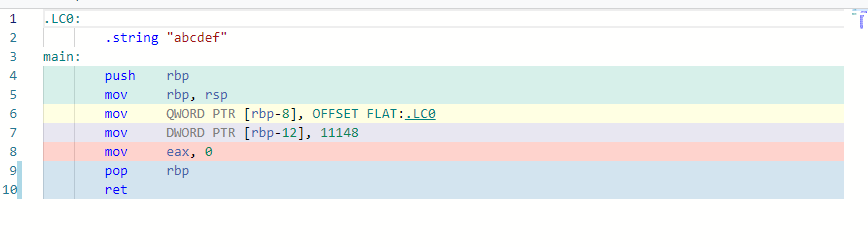
\includegraphics[width=.3\textwidth]{Imagenes/ejercicio 1.png}
		\end{center}
		Rpta: El segundo código da un error léxico en la linea 14 en el cual podemos ver que el variable no puede ser un numero por lo cual 4m no existe en el lenguaje. 
		\item Explique cual es la función del Scanner o Analizador Léxico. (2 puntos). \\
		Rpta: El analizador léxico se encarga de leer y de verificar que todo el código exista en el lenguaje. \newpage
		\item Dado el siguiente código, en una tabla escriba todos los Tokens que un Scanner encontraría ,detalle la clase y el lexema. Usted tiene la libertad de escoger el nombre de las clases. (4 puntos).
		\begin{center}
		     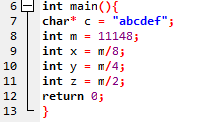
\includegraphics[width=.5\textwidth]{Imagenes/ejercicio 3.png}
		     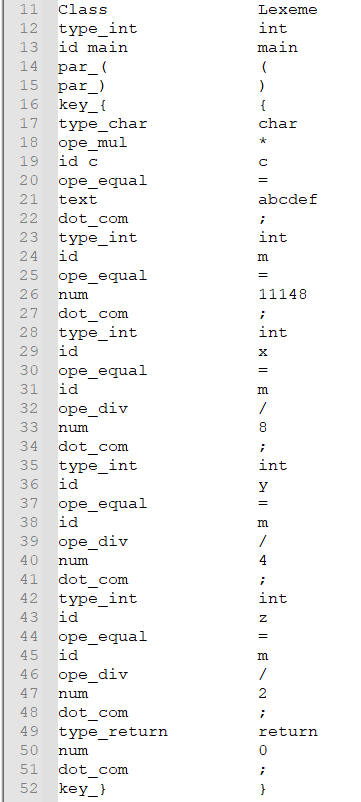
\includegraphics[width=.4\textwidth]{Imagenes/ejercicio 3.1.png}
		\end{center}
		\item Redacte el siguiente código en dos archivos distintos, luego compile cada archivo y explique a que se debe el tipo de error del segundo código. (2 puntos).
		\begin{center}
		     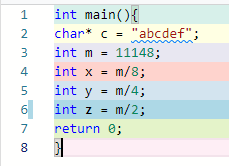
\includegraphics[width=.3\textwidth]{Imagenes/ejercicio 4.png}
		\end{center}
		Rpta: Hay un error sintáctico en la linea 14 done se puede ver que operación no se puede hacer por que falta un numero para sumar.
		\item Explique cual es la función  del Parser o Analizador Sintáctico. (2 puntos).\\
		 Rpta: El analizador, se encarga de analiza una cadena de símbolos según las reglas de una gramática formal.
		\item Genere el  árbol sintáctico para el siguiente código. Puede tomar como ejemplo el mostrado en clases. (4 puntos).
		\begin{center}
		     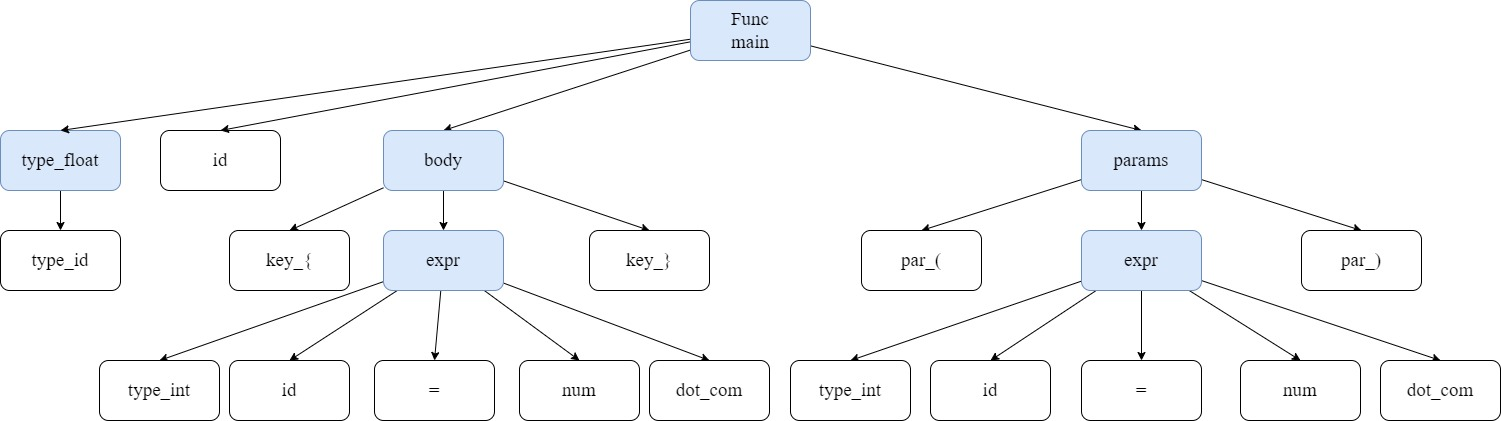
\includegraphics[width=.9\textwidth]{Imagenes/ejercicio 6.png}
		\end{center}
		\item Redacte el siguiente código en dos archivos distintos, luego compile cada archivo y explique a que se debe el tipo de error del segundo código. (2 puntos).
		\begin{center}
		     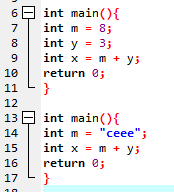
\includegraphics[width=.4\textwidth]{Imagenes/ejercicio 7.png}
		\end{center}
		Rpta: El error esta en la linea 14 es un error semántico, ya que se esta almacenando un char en una variable de tipo int. 
		\item Explique cual es la función del Analizador Semántico. (2 puntos).\\
		Rpta: El analizador semántico se verifica y analiza los tipos de datos y el ámbito de las variables.  

	\end{enumerate}


	
	%\clearpage
	%\bibliographystyle{apalike}
	%\bibliographystyle{IEEEtranN}
	%\bibliography{bibliography}
		
	
\end{document}